\documentclass{crypto-exercise}
\usepackage{amsthm}
\usepackage{graphics}
\usepackage{tikz}
\usetikzlibrary{trees}
\author{Sven Laur}
\contributor[Initial solution]{Karl Tarbe}
\contributor[Corrected several major errors]{Sven Laur}
\editor{Sven Laur}
\tags{sigma protocol, discrete logarithm, zero-knowledge, weak knowledge-extractor}

\begin{document}
\begin{exercise}{Weak knowledge-extractor for Schnorr protocol}
Let $\GG$ be a discrete logarithm group with a prime number $q$ elements. Show that the following knowledge-extractor constructor
\begin{align*}
\begin{fblock}{\KEXTR^{\PPP_*(\cdot)}(\phi)}
&\omega\gets\Omega\\
&\alpha\gets\PPP_*(\phi,\omega)\\
&\beta_1\getsu \ZZ_q\\
&\gamma_1\gets\PPP_*(\beta_1)\\
&\alpha\gets\PPP_*(\phi,\omega)\\
&\beta_2\getsu \ZZ_q\\
&\gamma_2\gets\PPP_*(\beta_2)\\
&\hat{x}\gets\frac{\gamma_2-\gamma_1}{\beta_2-\beta_1}\\
&\RETURN \hat{x}
\end{fblock}
\end{align*}
that restarts the prover with the same input and randomness only once is suitable for the Schnorr protocol \begin{center}
  \begin{tabular}{ccc}
    $\PPP$ & & $\VVV$\\
    $r\getsu\ZZ_q$ \\
    &$\xrightarrow{\makebox[6cm]{$\alpha=g^{r}$}}$ \\
    && $\beta\getsu\ZZ_q$ \\
    &$\xleftarrow{\makebox[6cm]{$\beta$}}$\\
    \\  
    &$\xrightarrow{\makebox[6cm]{$\gamma= x\beta+r$}}$\\
    && $\bigl[g^{\gamma}\iseq \alpha y^{\beta}\bigr]$\\  
  \end{tabular}
\end{center}  
and satisfies the following weak knowledge-extraction guarantee:
\begin{align*}
\forall \phi\in\set{0,1}^*\, \forall x\in\ZZ_q:\quad  \pr{\smash{\KEXTR^{\PPP_*(\cdot)}(\phi)=1}}\geq \pr{\smash{\VVV^{\PPP_*(\phi)}(g^x)=1}}^2-\frac{1}{q}\enspace.
\end{align*} 
Estimate the running time of the knowledge extractor and show that Schnorr identification protocol is secure if the underlying group is $(t,\varepsilon)$-secure Diffie-Hellman group. 
\end{exercise}

\begin{solution}
For the proof let us first establish the weak knowledge-extraction bound and then use this bound for estimating the probability that a malicious prover without the explicit knowledge of $x$ will succeed in the Schnorr identification protocol on average over all possible values of $x$. 

\vspace*{2ex}
\noindent
\textsc{Weak knowledge-extraction.} Let $\varepsilon(\phi,x)$ denote the probability of successful deception for fixed $\phi$ and $x$, i.e., the function $\varepsilon(\phi,x)$ is defined as follows
\begin{align*}
\varepsilon(\phi,x)=\pr{\smash{\VVV^{\PPP_*(\phi)}(g^x)=1}}=\pr{\alpha\gets\PPP_*(\phi),\beta\getsu\ZZ_q, \gamma\gets\PPP_*(\beta): g^\gamma=\alpha y^\beta}\enspace.
\end{align*}
Now lets look what has to happen for the knowledge extractor to succeed. The extraction succeeds only if both transcripts produced by $\KEXTR$ are valid and $\beta_1 \neq \beta_2$. If one of those conditions is not met, the extraction might succeed due to share luck but we cannot count on it. See the event tree depicted below.
 
\begin{center} 
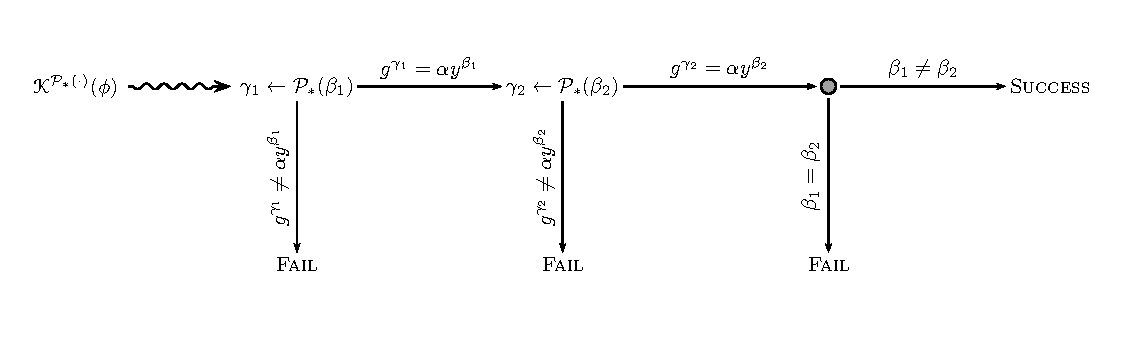
\includegraphics[scale=0.90, trim = 0cm 1cm 0cm 0.5cm, clip]{./figures/0908-event-tree}
\end{center}
As $\KEXTR$ executes two independent protocol runs between honest verifier and malicious prover $\PPP_*$
\begin{align*}
\pr{g^{\gamma_1}=\alpha y^{\beta_1}}=\varepsilon(\phi,x)=\pr{g^{\gamma_2}=\alpha y^{\beta_2}}\enspace.
\end{align*}
It is important to note that the event $[\beta_1\neq \beta_2]$ is not independent of the  event 
$[g^{\gamma_1}=\alpha y^{\beta_1}]\wedge [g^{\gamma_2}=\alpha y^{\beta_2}]$. For instance, the prover might succeed only if $\beta_i=0$ then obviously $\beta_1\neq\beta_2$ can be never met when the event  
$[g^{\gamma_1}=\alpha y^{\beta_1}]\wedge [g^{\gamma_2}=\alpha y^{\beta_2}]$ occurs while the event $\beta_1\neq\beta_2$ is quite probable without restrictions:
\begin{align*}
\pr{\beta_1\neq\beta_2|g^{\gamma_1}=\alpha y^{\beta_1}\wedge g^{\gamma_2}=\alpha y^{\beta_2}}\neq \pr{\beta_1\neq\beta_2}
\end{align*}
Consequently, we cannot use the standard decomposition for estimating the success:
\begin{align*}
    \pr{\textsc{Success}} = \varepsilon(\phi,x) \varepsilon(\phi,x)\pr{\beta_1\neq\beta_2|g^{\gamma_1}=\alpha y^{\beta_1}\wedge g^{\gamma_2}=\alpha y^{\beta_2}}\enspace,
\end{align*}
since we have no idea how to lower bound the last conditional probability. Thus, we have to rely on much cruder formula
\begin{align*}
    \pr{\textsc{Success}} =\pr{g^{\gamma_1}=\alpha y^{\beta_1}}  \pr{g^{\gamma_2}=\alpha y^{\beta_2}\wedge\beta_1\neq\beta_2|g^{\gamma_1}=\alpha y^{\beta_1}}\enspace.
\end{align*}
Due to the basic property of probabilities
\begin{align*}
\pr{A\wedge B}\geq\pr{A}-\pr{\neg B}
\end{align*}
we can lower bound the second term
\begin{align*}
\pr{g^{\gamma_2}=\alpha y^{\beta_2}\wedge\beta_1\neq\beta_2|g^{\gamma_1}=\alpha y^{\beta_1}}\geq \pr{g^{\gamma_2}=\alpha y^{\beta_2}|g^{\gamma_1}=\alpha y^{\beta_1}}- \pr{\beta_1=\beta_2|g^{\gamma_1}=\alpha y^{\beta_1}}\enspace.
\end{align*} 
The latter allows us to proceed as by the construction the event $[g^{\gamma_2}=\alpha y^{\beta_2}]$ is independent of $[g^{\gamma_1}=\alpha y^{\beta_1}]$. Similarly the event $[\beta_1=\beta_2]$ is independent of  $[g^{\gamma_1}=\alpha y^{\beta_1}]$. Consequently, we get
\begin{align*}
\pr{g^{\gamma_2}=\alpha y^{\beta_2}\wedge\beta_1\neq\beta_2|g^{\gamma_1}=\alpha y^{\beta_1}}
&\geq \pr{g^{\gamma_2}=\alpha y^{\beta_2}}- \pr{\beta_1=\beta_2}\geq\varepsilon(\phi,x)-\frac{1}{q}
\end{align*}
and 
\begin{align*}
\pr{\smash{\KEXTR^{\PPP_*(\cdot)}(\phi)=1}}\geq\pr{\textsc{Success}}\geq \varepsilon(\phi,x)\biggl(\varepsilon(\phi,x)-\frac{1}{q}\biggr)\geq \varepsilon(\phi,x)^2-\frac{1}{q}\enspace.
\end{align*}
As a result, we have proved the desired claim
\begin{align*}
 \forall \phi\in\set{0,1}^*\, \forall x\in\ZZ_q:\quad
    \pr{\smash{\KEXTR^{\PPP_*(\cdot)}(\phi)=1}}\geq \varepsilon(\phi, x)^2 -
    \frac{1}{q} = \pr{\smash{\VVV^{\PPP_*(\phi)}(g^x)=1}}^2 - \frac{1}{q} \enspace.
\end{align*}


\vspace*{2ex}
\noindent
\textsc{Security.} Let $\varepsilon(\phi)$ denote the average success rate of a malicious prover $\PPP_*$ that does not have access to the uniformly chosen exponent $x$. Then the weak knowledge extractor succeeds with the average probability
\begin{align*}
    \pr{\smash{x\getsu\ZZ_q:\KEXTR^{\PPP_*(\cdot)}(\phi,x)=1}}
    &=\sum_{x\in\ZZ_q}\frac{1}{q}\cdot \pr{\KEXTR^{\PPP_*(\cdot)}(\phi,x)=1}\\
    &\geq \sum_{x\in\ZZ_q}\frac{1}{q}\cdot 
      \biggl(\pr{\smash{\VVV^{\PPP_*(\phi)}(g^x)=1}}^2 - \frac{1}{q}\biggr)\\
    &\geq  \sum_{x\in\ZZ_q}\frac{1}{q}\cdot \pr{\smash{\VVV^{\PPP_*(\phi)}(g^x)=1}}^2-\frac{1}{q}\enspace. 
\end{align*}
As squaring is convex-cup function, we can apply Jensen's inequality 
\begin{align*}
    \pr{\smash{x\getsu\ZZ_q:\KEXTR^{\PPP_*(\cdot)}(\phi)=1}}
    &\geq  \Biggl(\sum_{x\in\ZZ_q}\frac{1}{q}\cdot \pr{\smash{\VVV^{\PPP_*(\phi)}(g^x)=1}}\Biggr)^2-\frac{1}{q}\geq \varepsilon(\phi)^2-\frac{1}{q}\enspace. 
\end{align*}
The latter gives us handle to limit the average success $\varepsilon(\phi)$. Recall that the security of discrete logarithm problem is defined through the following game:
\begin{align*}
\begin{fblock}{\BGAME}
&x\getsu\ZZ_q\\
&\RETURN \smash{[\ADB(g,g^x) \iseq x ]}\enspace.
\end{fblock}
\end{align*}
If the weak knowledge extractor has reasonable success peobability, we can use it as an adversary against discrete logarithm problem:
\begin{align*}
\begin{fblock}{\ADB(g,g^x)}
&\phi\gets(g,g^x)\\
&\RETURN \KEXTR^{\PPP_*(\cdot)}(\phi)\\
\end{fblock}
\end{align*}
By the construction, the running time of $\ADB$ is $2t_\PPP + \Oh(1)$, where $t_\PPP$ is
the running time of malicious prover $\PPP_*$ and the advantage against discrete logarithm is
\begin{align*}
\ADVDL{\GG}{\ADB}\geq \pr{x\gets\ZZ_q:\smash{\VVV^{\PPP_*(\phi)}(g^x)=1}}^2-\frac{1}{q}\enspace.
\end{align*}
By imitting constant terms, we obtain the following security claim. If the underlying DL group is $(t,\varepsilon)$-secure then Schnorr
identification protocol is
$\bigl(\frac{t}{2},\sqrt{\varepsilon+\frac{1}{q}}\bigr)$-secure.

\vspace*{2ex}
\noindent
\textsc{Comment on the security proof.} The presented reduction is not unique, as we could to $\ell$ rewindings instead of two in the weak knowledge extractor. Each choice of $\ell$ provides a different security guarantee. However, these are not directly comparable as the bounds on running times are different. Still, one could utilise all of them if instead of single security assumption $(t,\varepsilon)$ we look hypothetical success profile:
\begin{align*}
\varepsilon(t)=\max_{\ADB\text{is $t$-time}} \ADVDL{\GG}{\ADB}\enspace.
\end{align*}  
The result would be several competing upper bounds $\varepsilon_\ell^*(t)$ on the maximal average success against the Schnorr protocol on average. By combining them all we get a better bound. 

\end{solution}
\end{document}
